\documentclass{article} % For LaTeX2e
\usepackage{nips13submit_e,times}
\usepackage{hyperref}
\usepackage{cleveref}
\usepackage{graphicx}
\usepackage{url}
\usepackage{placeins}
\usepackage{fancyvrb}
\usepackage[font={small,it},width=5in]{caption}
%\documentstyle[nips13submit_09,times,art10]{article} % For LaTeX 2.09


\title{Musical Structure in Irish Traditional Tunes}

\author{Matthew Staib, Lennart Jansson, and Edward Dai}

% The \author macro works with any number of authors. There are two commands
% used to separate the names and addresses of multiple authors: \And and \AND.
%
% Using \And between authors leaves it to \LaTeX{} to determine where to break
% the lines. Using \AND forces a linebreak at that point. So, if \LaTeX{}
% puts 3 of 4 authors names on the first line, and the last on the second
% line, try using \AND instead of \And before the third author name.

\newcommand{\fix}{\marginpar{FIX}}
\newcommand{\new}{\marginpar{NEW}}

\nipsfinalcopy % Uncomment for camera-ready version

\begin{document}

\maketitle

\section{Introduction}
Most folk dance music contains two musical themes; the tune begins with one
musical theme which is usually repeated, then progresses to another theme with
similar musical structure and motives, which is usually also repeated. The first
section is typically called the $A$ section while the second is called the $B$
section. Our goal is to understand, at a quantitative level, the relationship
between $A$ sections and $B$ sections. In the long term, for example, we want to
be able to, given an $A$ section, automatically generate a musically appropriate
$B$ section.

In working towards this goal, we need to understand both the relationship
between the $A$ and $B$ section of a given folk song as well as the differences
between $A$ and $B$ sections of such music in general. 

\section{Dataset}

We are using the tunes dataset from The Session (\texttt{thesession.org}). The
Session is an online community of people who are interested in playing Irish
folk music and cataloguing traditional Irish tunes for others to learn. These
tunes include various dance forms, such as jigs, reels, waltzes, and slides.
Available on their website is a set of roughly 21 thousand dance tune settings
in ABC notation, a human-readable symbolic music data format in plain text. The
ABC files are easily parsed and manipulated symbolically for feature extraction.
\FloatBarrier
\begin{figure}[t]
  \begin{center}
  \begin{BVerbatim}
X: 1
T: Drowsy Maggie
R: reel
M: 4/4
L: 1/8
K:Edor
|:E2BE dEBE|E2BE AFDF|E2BE dEBE|BABc dAFD:|
K:D
d2fd c2ec|defg afge|d2fd c2ec|BABc dAFA|
d2fd c2ec|defg afge|afge fdec|BABc dAFD|
  \end{BVerbatim}
  \end{center}
  \caption{\textit{Drowsy Maggie}, an example of a tune in ABC notation from
  \texttt{thesession.org}.}
\end{figure}

\begin{figure}[t]
  \begin{center}
    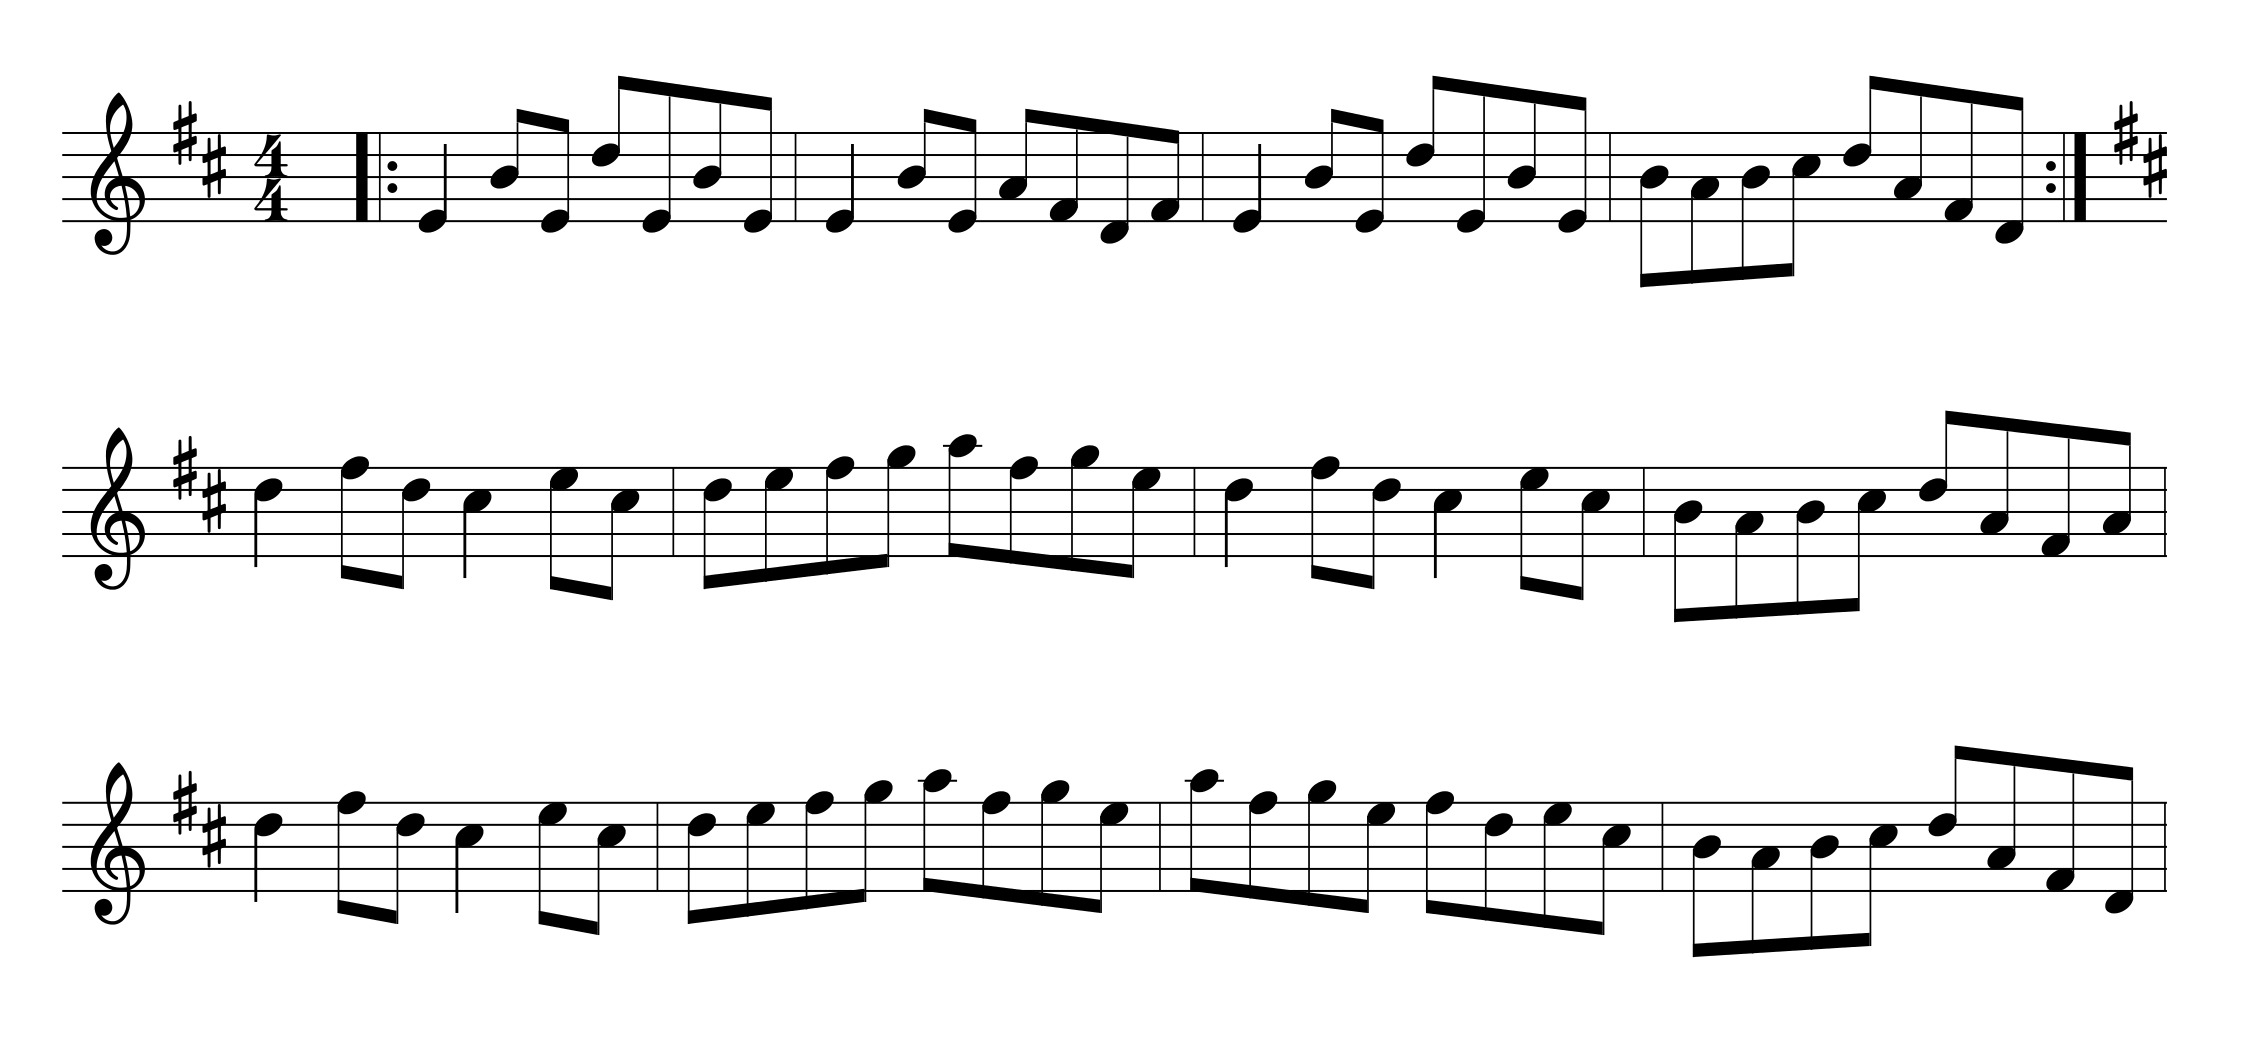
\includegraphics[width=5in]{drowsymaggie.png}
  \end{center}
  \caption{A rendering of \textit{Drowsy Maggie} in standard musical notation, for
  comparison with ABC notation. The $A$ section of this tune can be seen in the
first line, while the $B$ section spans the second and third lines. The $A$ and
$B$ sections are the same length since the first four bars are repeated---both
are eight bars long when performed. Note that this tune, like many others, has
four-bar phrases, which supports the heuristic we are using for splitting into
$A$ and $B$ sections.}
  \label{fig:drowsymusic}
\end{figure}
%\FloatBarrier

\section{Feature Extraction}

%We first use an ABC parser to turn the tunes in ABC notation into manipulable
%datatypes of bars and notes. For feature extraction, we count frequencies of
%$n$-grams of note pitches up to $n=3$, which gives information about the
%characteristic pitch contours of the individual tunes.
%
%We are not currently using rhythm information of notes, nor are we considering
%the particular octave or accidental inflection of pitches. This is a very basic
%feature extraction scheme and we hope to extend our feature extraction soon to
%include this other information, which may be useful in improving accuracy of our
%classifiers.
%
%For our work with $A$ and $B$ section classification and matching, we use a
%simple heuristic to split tunes into $A$ and $B$ sections as they are not
%explicitly labelled in the data set. We first unfold all symbolic repeats in the
%original tune, taking into consideration 1st and 2nd endings which very commonly
%appear at the end of both $A$ and $B$ sections. This produces continuous streams
%of music that are more easily analyzed, and reflect the structure of the tune as
%it sounds when performed, rather than how it appears in notation.
%
%Then, if the tune has a number of bars that is a multiple of 4, we split the
%tune evenly in half. This is an imprecise heuristic, but should work well in
%practice because $A$ and $B$ sections generally have the same number of bars as
%they most commonly have parallel musical structure, and also because these
%traditional tunes most commonly have 4-bar phrases within $A$ and $B$ sections.
%See \cref{fig:drowsymusic} for an example.
%

\end{document}
